% xcolor and define colors -------------------------
\usepackage{xcolor}

% https://www.viget.com/articles/color-contrast/
\definecolor{purple}{HTML}{5601A4}
\definecolor{navy}{HTML}{0D3D56}
\definecolor{ruby}{HTML}{9a2515}
\definecolor{alice}{HTML}{107895}
\definecolor{daisy}{HTML}{EBC944}
\definecolor{coral}{HTML}{F26D21}
\definecolor{kelly}{HTML}{829356}
\definecolor{cranberry}{HTML}{E64173}
\definecolor{jet}{HTML}{131516}
\definecolor{asher}{HTML}{555F61}
\definecolor{slate}{HTML}{314F4F}

% Mixtape Sessions
\definecolor{picton-blue}{HTML}{00b7ff}
\definecolor{violet-red}{HTML}{ff3881}
\definecolor{sun}{HTML}{ffaf18}
\definecolor{electric-violet}{HTML}{871EFF}

\newcommand\pictonBlue[1]{{\color{picton-blue}#1}}
\newcommand\sun[1]{{\color{sun}#1}}
\newcommand\electricViolet[1]{{\color{electric-violet}#1}}
\newcommand\violetRed[1]{{\color{violet-red}#1}}

\newcommand\bgPictonBlue[1]{{\colorbox{picton-blue!20!white}{#1}}}
\newcommand\bgSun[1]{{\colorbox{sun!20!white}{#1}}}
\newcommand\bgElectricViolet[1]{{\colorbox{electric-violet!20!white}{#1}}}
\newcommand\bgVioletRed[1]{{\colorbox{violet-red!20!white}{#1}}}

\def\code#1{\texttt{#1}}

% Main theme colors
\definecolor{accent}{HTML}{00b7ff}
\definecolor{accent2}{HTML}{871EFF}
\definecolor{gray100}{HTML}{f3f4f6}
\definecolor{gray800}{HTML}{1F292D}


% Beamer Options -------------------------------------

% Background
\setbeamercolor{background canvas}{bg = white}

% Change text margins
\setbeamersize{text margin left = 15pt, text margin right = 15pt} 

% \alert
\setbeamercolor{alerted text}{fg = accent2}

% Frame title
\setbeamercolor{frametitle}{bg = white, fg = jet}
\setbeamercolor{framesubtitle}{bg = white, fg = accent}
\setbeamerfont{framesubtitle}{size = \small, shape = \itshape}

% Block
\setbeamercolor{block title}{fg = white, bg = accent2}
\setbeamercolor{block body}{fg = gray800, bg = gray100}

% Title page
\setbeamercolor{title}{fg = gray800}
\setbeamercolor{subtitle}{fg = accent}

%% Custom \maketitle and \titlepage
\setbeamertemplate{title page}
{
    %\begin{centering}
        \vspace{20mm}
        {\Large \usebeamerfont{title}\usebeamercolor[fg]{title}\inserttitle}\\
        {\large \itshape \usebeamerfont{subtitle}\usebeamercolor[fg]{subtitle}\insertsubtitle}\\ \vspace{10mm}
        {\insertauthor}\\
        {\color{asher}\small{\insertdate}}\\
    %\end{centering}
}

% Table of Contents
\setbeamercolor{section in toc}{fg = accent!70!jet}
\setbeamercolor{subsection in toc}{fg = jet}

% Button 
\setbeamercolor{button}{bg = accent}

% Remove navigation symbols
\setbeamertemplate{navigation symbols}{}

% Table and Figure captions
\setbeamercolor{caption}{fg=jet!70!white}
\setbeamercolor{caption name}{fg=jet}
\setbeamerfont{caption name}{shape = \itshape}

% Bullet points

%% Fix spacing between items
\let\olditemize=\itemize 
\let\endolditemize=\enditemize 
\renewenvironment{itemize}{\vspace{0.25em}\olditemize \itemsep0.25em}{\endolditemize}

%% Fix left-margins
\settowidth{\leftmargini}{\usebeamertemplate{itemize item}}
\addtolength{\leftmargini}{\labelsep}

%% enumerate item color
\setbeamercolor{enumerate item}{fg = accent}
\setbeamerfont{enumerate item}{size = \small}
\setbeamertemplate{enumerate item}{\insertenumlabel.}

%% itemize
\setbeamercolor{itemize item}{fg = accent!70!white}
\setbeamerfont{itemize item}{size = \small}
\setbeamertemplate{itemize item}[circle]

%% right arrow for subitems
\setbeamercolor{itemize subitem}{fg = accent!60!white}
\setbeamerfont{itemize subitem}{size = \small}
\setbeamertemplate{itemize subitem}{$\rightarrow$}

\setbeamertemplate{itemize subsubitem}[square]
\setbeamercolor{itemize subsubitem}{fg = jet}
\setbeamerfont{itemize subsubitem}{size = \small}








% Links ----------------------------------------------

\usepackage{hyperref}
\hypersetup{
  colorlinks = true,
  linkcolor = accent2,
  filecolor = accent2,
  urlcolor = accent2,
  citecolor = accent2,
}


% Line spacing --------------------------------------
\usepackage{setspace}
\setstretch{1.35}


% \begin{columns} -----------------------------------
\usepackage{multicol}


% Fonts ---------------------------------------------
% Beamer Option to use custom fonts
\usefonttheme{professionalfonts}

% \usepackage[utopia, smallerops, varg]{newtxmath}
% \usepackage{utopia}
\usepackage[sfdefault,light]{roboto}

% Small adjustments to text kerning
\usepackage{microtype}



% Remove annoying over-full box warnings -----------
\vfuzz2pt 
\hfuzz2pt


% Table of Contents with Sections
\setbeamerfont{myTOC}{series=\bfseries, size=\Large}
\AtBeginSection[]{
        \frame{
            \frametitle{Roadmap}
            \tableofcontents[current]   
        }
    }


% Tables -------------------------------------------
% Tables too big
% \begin{adjustbox}{width = 1.2\textwidth, center}
\usepackage{adjustbox}
\usepackage{array}
\usepackage{threeparttable, booktabs, adjustbox}
    
% Fix \input with tables
% \input fails when \\ is at end of external .tex file
\makeatletter
\let\input\@@input
\makeatother

% Tables too narrow
% \begin{tabularx}{\linewidth}{cols}
% col-types: X - center, L - left, R -right
% Relative scale: >{\hsize=.8\hsize}X/L/R
\usepackage{tabularx}
\newcolumntype{L}{>{\raggedright\arraybackslash}X}
\newcolumntype{R}{>{\raggedleft\arraybackslash}X}
\newcolumntype{C}{>{\centering\arraybackslash}X}

% Figures

% \imageframe{img_name} -----------------------------
% from https://github.com/mattjetwell/cousteau
\newcommand{\imageframe}[1]{%
    \begin{frame}[plain]
        \begin{tikzpicture}[remember picture, overlay]
            \node[at = (current page.center), xshift = 0cm] (cover) {%
                \includegraphics[keepaspectratio, width=\paperwidth, height=\paperheight]{#1}
            };
        \end{tikzpicture}
    \end{frame}%
}

% subfigures
\usepackage{subfigure}


% Highlight slide -----------------------------------
% \begin{transitionframe} Text \end{transitionframe}
% from paulgp's beamer tips
\newenvironment{transitionframe}{
    \setbeamercolor{background canvas}{bg=accent!40!black}
    \begin{frame}\color{accent!10!white}\LARGE\centering
}{
    \end{frame}
}


% Table Highlighting --------------------------------
% Create top-left and bottom-right markets in tabular cells with a unique matching id and these commands will outline those cells
\usepackage[beamer,customcolors]{hf-tikz}
\usetikzlibrary{calc}
\usetikzlibrary{fit,shapes.misc}

% To set the hypothesis highlighting boxes red.
\newcommand\marktopleft[1]{%
    \tikz[overlay,remember picture] 
        \node (marker-#1-a) at (0,1.5ex) {};%
}
\newcommand\markbottomright[1]{%
    \tikz[overlay,remember picture] 
        \node (marker-#1-b) at (0,0) {};%
    \tikz[accent!80!jet, ultra thick, overlay, remember picture, inner sep=4pt]
        \node[draw, rectangle, fit=(marker-#1-a.center) (marker-#1-b.center)] {};%
}


% DAGS ----------------------------------------------
\usepackage{tikz}
\usetikzlibrary{shapes,decorations,arrows,calc,arrows.meta,fit,positioning}
% Tikz settings optimized for causal graphs.
\tikzset{
    -Latex,auto,node distance =1 cm and 1 cm,semithick,
    state/.style ={ellipse, draw, minimum width = 0.7 cm},
    point/.style = {circle, draw, inner sep=0.04cm,fill,node contents={}},
    bidirected/.style={Latex-Latex,dashed},
    el/.style = {inner sep=2pt, align=left, sloped}
}


% Beamer tricks -------------------------------------
% Make \pause work in align environments
\makeatletter
\renewrobustcmd{\beamer@@pause}[1][]{%
  \unless\ifmeasuring@%
  \ifblank{#1}%
    {\stepcounter{beamerpauses}}%
    {\setcounter{beamerpauses}{#1}}%
  \onslide<\value{beamerpauses}->\relax%
  \fi%
}
\makeatother


\title [Nonparametrics]{Nonparametrics and Local Methods: Polynomials}
\author{C.Conlon}
\institute{Applied Econometrics}
\date{\today}
\setbeamerfont{equation}{size=\tiny}
\begin{document}

\begin{frame}
\titlepage
\end{frame}

\begin{frame}{Polynomial Basis}
Again consider the following relationship:
\begin{align*}
y_i = f(x_i) + \epsilon_i
\end{align*}
One approach is to approximate $f(x_i)$ or $E[y_i | x_i]$ with a \alert{polynomial series}.
\begin{align*}
y_i = a_0  + a_1 x_i + a_2 x_i^2 + a_3 x_i^3+ \cdots+ a_M x_i^M + \varepsilon_i
\end{align*}
An important choice is to choose polynomial order $M$ (complexity)\\
Idea: we can approximate \alert{arbitrary (smooth) functions} $f(x_i)$ with a high-order polynomial.
\end{frame}

\begin{frame}{Polynomial Example}
Let's suppose we want to approximate the following function:
\begin{align*}
\frac{1}{3} \sin (2 x) \approx \frac{2}{3} x - \frac{4}{9} x^3 + \frac{4}{45} x^5 + O(x^7)
\end{align*}
This should be easy since we have a \alert{Taylor Expansion} that is polynomial in $x$ (also it is odd).
\end{frame}

\begin{frame}[fragile]{Polynomial Example}
\begin{columns}
\begin{column}{0.5\textwidth}
 \tiny
\begin{verbatim}
library(ggplot2)    

# set the seed to make the results reproducible.
set.seed(3)







#### simulate some data ####
# epsilon = random error term
epsilon <- 0.25*rnorm(100)
x       <- seq(from=1, to=5, length.out=100)
y       <- 1 +sin(x*2)/3 + epsilon





# visualize the data (with a polynomial best-fit line)
ggplot(data=NULL,aes(x, y)) + geom_point() + 
geom_smooth(method = "lm", formula = y ~ poly(x, 3,raw=T),color='maroon')+
geom_smooth(method = "lm", formula = y ~ poly(x, 5,raw=T),color='navy')+
geom_smooth(method = "lm", formula = y ~ poly(x, 17,raw=T),color='darkgreen')
\end{verbatim}
\end{column}
\begin{column}{0.5\textwidth}  %%<--- here
    \begin{center}
    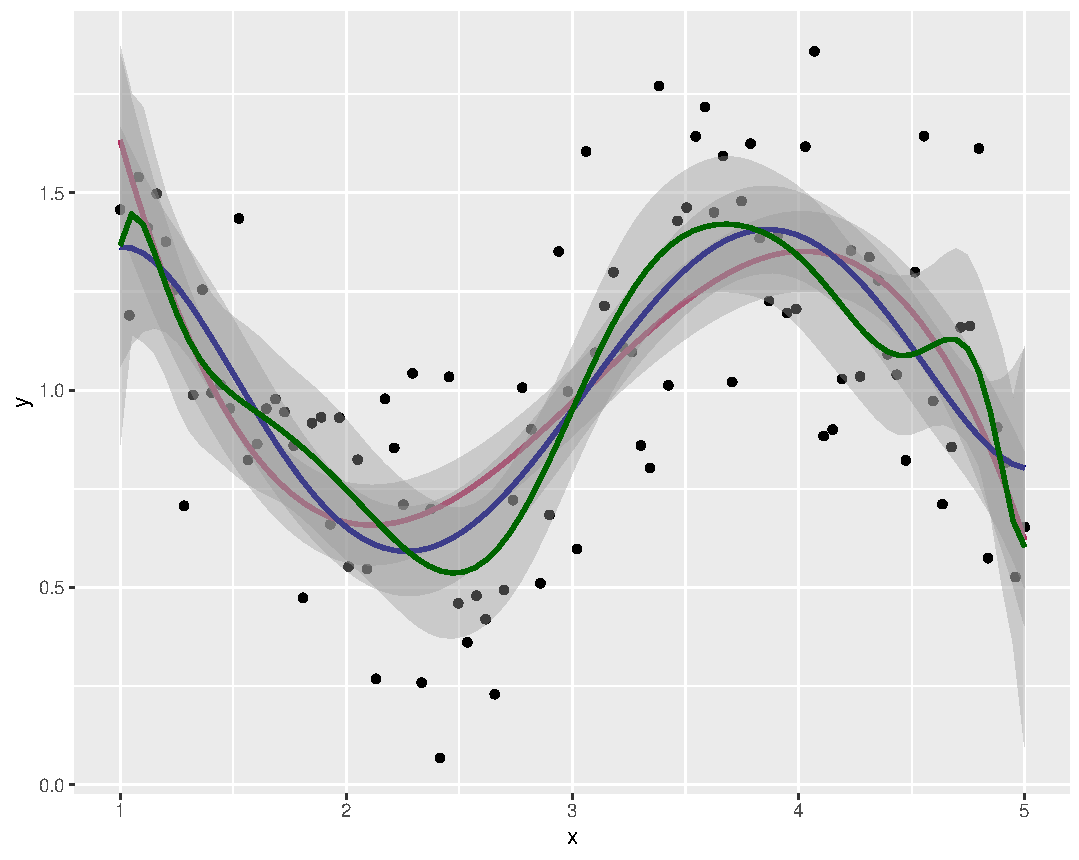
\includegraphics[width=\textwidth]{./resources/poly.pdf}
     \end{center}
\end{column}
\end{columns}
\end{frame}

\begin{frame}[fragile]{Polynomial Example}
\begin{itemize}
\item $M=5$ order polynomial should fit the data well (it does).
\item We are clearly \alert{overfitting} at $M=17$ since this doesn't look much like $y(x) = \sin(2x)/3 + \varepsilon$.
\item We used \alert{raw polynomials}: $x,x^2,x^3,\ldots$.
\item By default R uses \alert{orthogonal polynomials} when we drop \texttt{raw=TRUE}.\\
(More on these later)
\end{itemize}
\tiny 
\begin{verbatim}
# visualize the data (with a polynomial best-fit line)
ggplot(data=NULL,aes(x, y)) + geom_point() + 
geom_smooth(method = "lm", formula = y ~ poly(x, 3),color='maroon')+
geom_smooth(method = "lm", formula = y ~ poly(x, 5),color='navy')+
geom_smooth(method = "lm", formula = y ~ poly(x, 17),color='darkgreen')
\end{verbatim}
\end{frame}

\begin{frame}[fragile]{``Raw'' Polynomials}
\begin{columns}
\begin{column}{0.6\textwidth}
\tiny
\begin{verbatim}
                          Estimate Std. Error t value Pr(>|t|)
(Intercept)              -5.421717   8.009814  -0.677    0.500
poly(x, 6, raw = T)1  18.072018  20.371055   0.887    0.377
poly(x, 6, raw = T)2 -17.392013  20.363051  -0.854    0.395
poly(x, 6, raw = T)3   7.503790  10.288970   0.729    0.468
poly(x, 6, raw = T)4  -1.561290   2.786268  -0.560    0.577
poly(x, 6, raw = T)5   0.148442   0.385418   0.385    0.701
poly(x, 6, raw = T)6  -0.004826   0.021378  -0.226    0.822
\end{verbatim}

\begin{verbatim}
                          Estimate Std. Error t value Pr(>|t|)   
(Intercept)               45.71304   19.95109   2.291  0.02423 * 
poly(x, 7, raw = TRUE)1 -138.78101   59.74402  -2.323  0.02239 * 
poly(x, 7, raw = TRUE)2  177.80275   72.90420   2.439  0.01665 * 
poly(x, 7, raw = TRUE)3 -120.61050   47.13566  -2.559  0.01214 * 
poly(x, 7, raw = TRUE)4   46.52356   17.50188   2.658  0.00926 **
poly(x, 7, raw = TRUE)5  -10.21667    3.74637  -2.727  0.00765 **
poly(x, 7, raw = TRUE)6    1.18842    0.42965   2.766  0.00686 **
poly(x, 7, raw = TRUE)7   -0.05682    0.02044  -2.780  0.00658 **
\end{verbatim}
\end{column}
\begin{column}{0.4\textwidth}
\begin{itemize}
\item 6th order polynomial: nothing significant
\item 7th order polynomial: all terms significant (odd and even).
\item Totally different coefficients!
\item Both highly sensitive to small changes in $x_i$.
\end{itemize}
\end{column}
\end{columns}
\end{frame}


\begin{frame}[fragile]{``Orthogonal'' Polynomials}
\begin{columns}
\begin{column}{0.6\textwidth}
\tiny
\begin{verbatim}
                         Estimate Std. Error t value Pr(>|t|)    
(Intercept)               1.02278    0.02779  36.803  < 2e-16 ***
poly(x, 6, raw = FALSE)1  0.64772    0.27791   2.331  0.02193 *  
poly(x, 6, raw = FALSE)2  0.48158    0.27791   1.733  0.08643 .  
poly(x, 6, raw = FALSE)3 -2.47613    0.27791  -8.910 4.14e-14 ***
poly(x, 6, raw = FALSE)4 -0.16435    0.27791  -0.591  0.55571    
poly(x, 6, raw = FALSE)5  0.79114    0.27791   2.847  0.00543 ** 
poly(x, 6, raw = FALSE)6 -0.06273    0.27791  -0.226  0.82190    
\end{verbatim}

\begin{verbatim}
                         Estimate Std. Error t value Pr(>|t|)    
(Intercept)               1.02278    0.02684  38.111  < 2e-16 ***
poly(x, 7, raw = FALSE)1  0.64772    0.26837   2.414  0.01778 *  
poly(x, 7, raw = FALSE)2  0.48158    0.26837   1.794  0.07602 .  
poly(x, 7, raw = FALSE)3 -2.47613    0.26837  -9.227 9.68e-15 ***
poly(x, 7, raw = FALSE)4 -0.16435    0.26837  -0.612  0.54179    
poly(x, 7, raw = FALSE)5  0.79114    0.26837   2.948  0.00405 ** 
poly(x, 7, raw = FALSE)6 -0.06273    0.26837  -0.234  0.81569    
poly(x, 7, raw = FALSE)7 -0.74618    0.26837  -2.780  0.00658 ** 
\end{verbatim}
\end{column}
\begin{column}{0.4\textwidth}
\begin{itemize}
\item Odd terms are significant in both specifications
\item Coefficients appear stable (!)
\item Usually coefficients decline in (odd) polynomial order.
\item But very high dimensional polynomials will still \alert{overfit}.
\end{itemize}
\end{column}
\end{columns}
\end{frame}

\begin{frame}{Orthgonal Polynomials}
Consider an arbitrary basis:
\begin{align*}
y(x_i) = a_0 + \sum_{j=1}^M a_j b_j(x_i) + \varepsilon_i
\end{align*}
\begin{itemize}
\item $ b_j(x_i) = x_i^j$ (regular polynomials)
\item $\langle b_j(x),b_k(x)  \rangle=0$ for $j \neq k$ (orthogonal polynomials).
\item Lots of options: Chebyshev, Legendre, Fourier, Gram Schmidt (discuss later).
\end{itemize}
\end{frame}

\begin{frame}{What R does: Gram Schmidt}
Let $a_j = x^j$ (the raw polynomial) and then \alert{orthogonalize} as follows:
\begin{align*}
\hat{p}_{j}(x)&=a_{j}(x)-\sum_{k=0}^{j-1} p_{k}(x) \frac{p_{k} \cdot a_{j}}{p_{k} \cdot p_{k}}, \quad 
p(x)=\frac{\hat{p}(x)}{ \hat{p}(1)}
\end{align*}
\begin{itemize}
\item We are forming the \alert{residual} of $x^j$ on $(x^{j-1}, x^{j-2},\ldots, x, 1)$ (where each term has already been residualized).
\item Notice, we don't need to know $y_i$, we can simply residualized $x_i$ against powers of itself.
\item We could do this for any matrix $X$! (doesn't need to be powers of $x_i$).
\end{itemize}
\end{frame}


\begin{frame}{Orthogonal Polynomials}
\small
\begin{block}{General Case}
\begin{itemize}
\item Space: polynomials over domain $D$
\item Weighting function: $w(x) > $ (positive everywhere)
\item Inner product $\langle f,g \rangle = \int_D f(x) g(x) w(x) d x$
\item Polynomials are orthogonal wrt to $w(x)$ IFF 
\begin{align*}
\langle \phi_i, \phi_j \rangle = 0, \quad i \neq j
\end{align*}
\item Can compute orthogonal polynomials using recurrence formulas
\begin{align*}
\phi_0(x)&= 1\\
\phi_1(x) &= x \\
\phi_{k+1}(x) &= (a_{k+1} x + b_k) \phi_k(x) + c_{k+1} \phi_{k-1}(x)
\end{align*}
\end{itemize}
\end{block}
\end{frame}

\begin{frame}{Chebyshev Polynomials}
\small
\begin{itemize}
\item Can compute orthogonal polynomials using recurrence formulas
\item $[a,b] = [-1,1]$ and $w(x) = (1-x^2)^{-1/2}$
\item $T_n(x) = \cos(n \cos^{-1} x)$
\item Recursive Definition 
\vspace{-1cm}
\begin{align*}
T_0(x) &= 1\\
T_1(x) &= x\\
T_{n+1}(x) &= 2x T_n(x) - T_{n-1}(x)
\end{align*}
\end{itemize}
\begin{block}{General Intervals}
\begin{itemize}
\item Most problems aren't on the $[-1,1]$ interval so we need a COV
\begin{align*}
y = -1 + 2 \frac{x-a}{b-a}
\end{align*}
\item Polynomials $\phi_i^{*}(x) \equiv \phi_i (-1 + 2 \frac{x-a}{b-a})$ are orthogonal over $x \in[a,b]$ with respect to the weight $w^{*}(x) \equiv (-1 + 2 \frac{x-a}{b-a})$ iff the $\phi_i(y)$ are orthogonal over $y\in[-1,1]$ wrt $w(y)$.
\end{itemize} 
\end{block}
\end{frame}

\begin{frame}{Chebyshev Approximation Algorithm}
\small
\begin{enumerate}
\item Compute the $m \geq n+1$ Chebyshev nodes on $[-1,1]$
\begin{eqnarray*}
z_k = -\cos \left ( \frac{2k-1}{2m} \pi \right) , \quad k=1,\ldots,m
\end{eqnarray*}
\item Adjust the nodes to $[a,b]$ interval
\begin{eqnarray*}
x_k = (z_k + 1)\left(\frac{b-a}{2} \right) + a , \quad k=1,\ldots,m
\end{eqnarray*}
\item Evaluate $f$ at the nodes $w_k = f(x_k)$ for $ k=1,\ldots,m$
\item Compute the coefficients $a_i$ to get the approximation $p(x)$
\begin{eqnarray*}
a_i = \frac{\sum_{k=1}^m w_k T_i(z_k)}{\sum_{k=1}^m  T_i(z_k)^2}, \quad
p(x) = \sum_{i=0}^n a_i T_i \left( 2 \frac{x-a}{b-a} -1 \right) 
\end{eqnarray*}
\end{enumerate}
\end{frame}

\begin{frame}{Minimax Approximation}
\begin{itemize}
\item Data: $(x_i,y_i)$, $i=1,\ldots,n$
\item Objective: $L^{\infty}$ fit
\begin{eqnarray*}
\min_{\beta \in R^m} \max_{i} \| y_i - f(x_i; \beta) \|
\end{eqnarray*}
\item Difficult to do (minimax problems are non-convex)
\item Chebyshev Approximation satisfies this property, for $C^2,C^3$ functions but doesn't get $f'(x)$ right!
\end{itemize}
\begin{theorem}
Suppose $f: [-1,1] \rightarrow R$ is $C^k$ for some $k \geq 1$, and let $I_n$ be the degree $n$ polynomial interpolation of $f$ based at the zeroes of $T_{n+1}(x)$ then
\begin{eqnarray*}
\tiny
\| f - I_n \|_{\infty} \leq \left(\frac{2}{\pi}  \log(n+1) + 1 \right) \frac{(n-k)!}{n!} \left ( \frac{\pi}{2}\right)^k  \left ( \frac{b-a}{2}\right)^k \| f^{(k)} \|_{\infty}
\end{eqnarray*}
\end{theorem}
\end{frame}

\begin{frame}{Recap: Polynomials}
\begin{align*}
y(x_i) = a_0 + \sum_{j=1}^M a_j b_j(x_i) + \varepsilon_i
\end{align*}
\begin{itemize}
\item Thus far have looked at \alert{global polynomial approximations}.
\item Global: basis $b_j(x)$ and coefficients $a_j$ are the same for any value of $x$.
\item Can choose polynomial order with \alert{cross validation}, later we will explore \alert{penalization}.
\item Special case of \alert{sieve estimators}: we let the order $M \rightarrow \infty$ as $n \rightarrow \infty$ but not as quickly!
\end{itemize}
\end{frame}



\end{document}